\section{Produktdaten}
Das Endprodukt muss für die erfolgreiche Verwendung auf einige Benutzerdaten zugreifen können und diese in manchen Fällen sogar verändern. Außerdem müssen Daten für den Transfer kurzzeitig gespeichert und mit dem Empfänger mit jedem Paket ausgetauscht werden.
\\
%\begin{comment}
\begin{figure}[H]
	\centering
	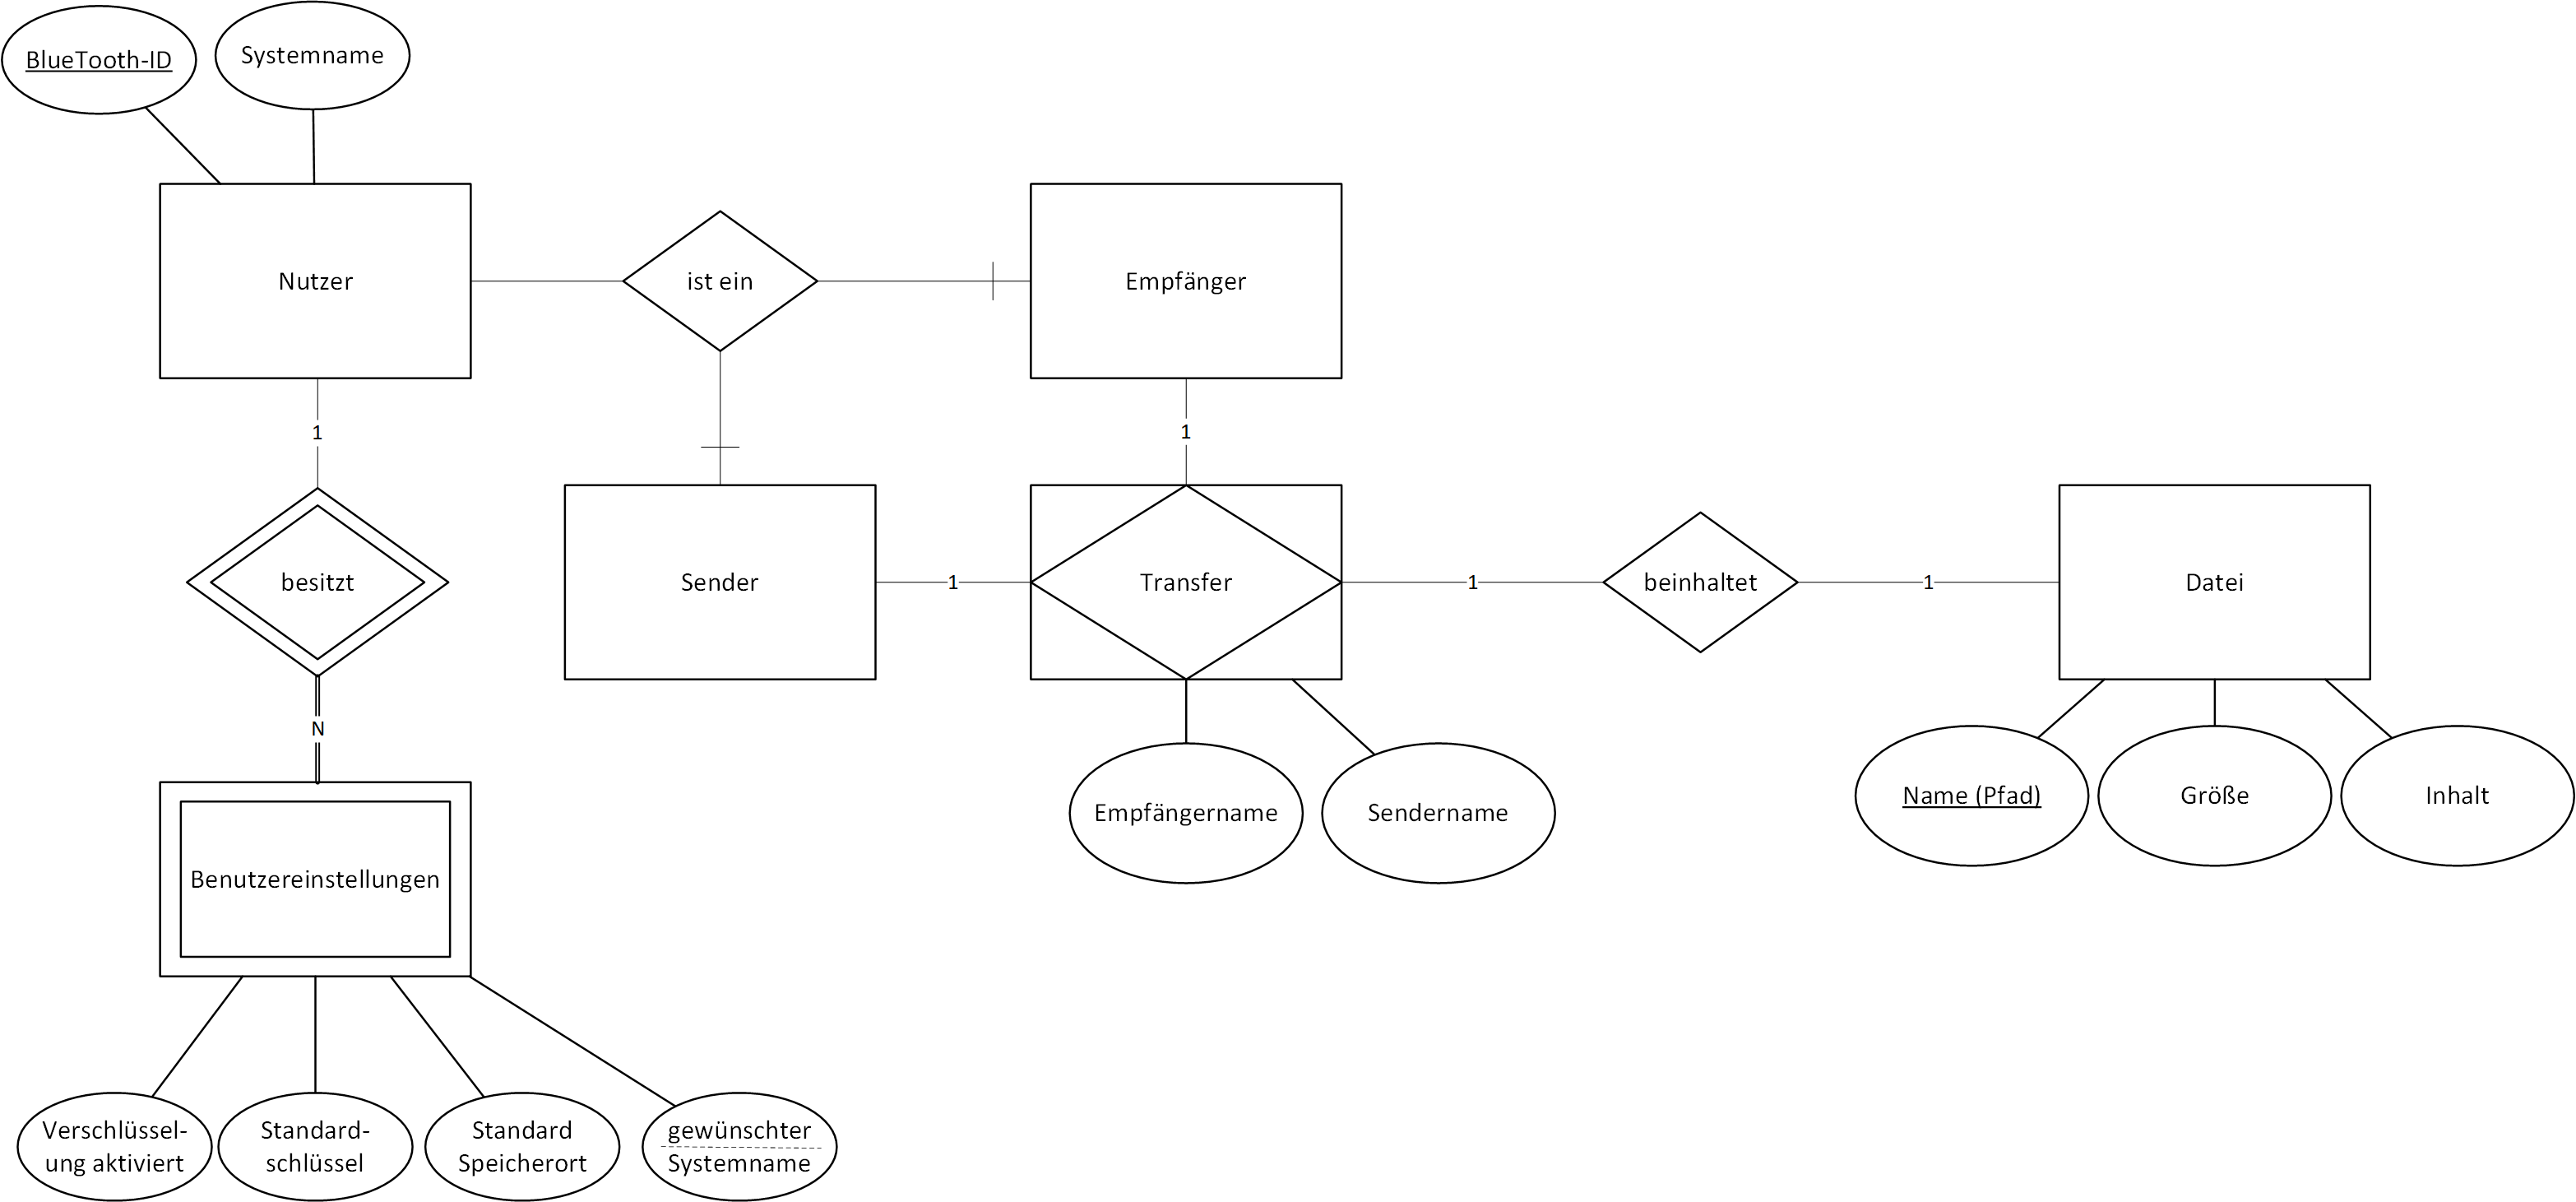
\includegraphics[width=\linewidth]{diagramms/erd/erd.png}\
	\caption{ERD}
\end{figure}
\newpage
%\end{comment}
\subsection{/LD1000/ Systemdaten}
\begin{itemize}
	\item momentaner-Systemname
	\item BlueTooth-Version
\end{itemize}
\subsection{/LD2000/ Datei}
\begin{itemize}
	\item Dateiname
	\item Dateigröße
	\item Dateiinhalt
\end{itemize}
\subsection{/LD3000/ Transferdaten}
\begin{itemize}
	\item Sendername
	\item Empfängername
	\item Datei
	\item Index Paket
	\item Anzahl Pakete
\end{itemize}
\subsection{/LD4000/ Benutzereinstellungen}
\begin{itemize}
	\item gewünschter Systemname
	\item Verschlüsselung (de- oder aktiviert)
	\item Standardschlüssel
	\item Standard-Speicherort
\end{itemize}